% !TEX root = ../main.tex
\section{Description of the Sample Application}
\label{sec:descr-sample-appl}

To illustrate the development and analysis process of a design using the previously described 
state-chart semantics, we will discuss a quadrotor helicopter or quadrotor application similar to 
the one presented by Syriani et al.~\cite{Syriani_2019}. 
The application will focus on the incremental design of some of the drone's required functionality.
The constructed model must obey state-chart refinement rules listed in Section~\ref{sec:intro}, these rules are proven within the Rodin tool.
The structure of the state-chart for this model at each subsequent abstraction level restricts further the development of the model to refinements that obey the rules. 
This will allow us to prove properties of the model in a very strategic fashion, as properties proven of early abstraction levels are preserved in later refinements.

The initial abstraction and first refinement of the model, shown in Figure~\ref{fig:drone1}, capture the basic functionality of the drone. 
The abstract model is shown in blue; the model's initial state is |OFF| and as a result of the |on| and  |toTakeoff| external triggers it transitions to the |START| and |OPERATIONAL| states respectively\footnote{Transitions in Figures~\ref{fig:drone1}--\ref{fig:drone4} are labeled with trigger names
(e.g.,toTakeoff, toFly) not with event names as it is in \UMLB.}. 
The drone reacts to the |off| external trigger by shutting down and subsequently transitioning to the |OFF| state.
The first refinement is constructed using \emph{Rule C}, which adds details within the |OPERATIONAL| state (gray states in Figure~\ref{fig:drone1}).
Within the |OPERATIONAL| state the drone will transition to |FLY| or |DESCEND| after the internal trigger |toFly| or |toLand| is raised, respectively. 
In refinement level one, these internal triggers are raised non-deterministically in the system by functionality not currently defined.
As additional details are incorporated into the model in later refinements some of that non-determinism is 
removed and replaced by transitions with actions that raised the previously defined internal triggers.
A further external trigger, |landed|, directs the system to progress to the |LANDED| state.
It should be noted that this abstraction of the drone model includes a transition from |TAKEOFF| to |DESCEND| (dashed transition in Figure~\ref{fig:drone1}). 
This allows for the drone to respond to a |toLand| trigger if it encounters some problems while in the |TAKEOFF| state.
Syriani et al.~\cite{Syriani_2019} introduces this transition in later refinements under Rule 8 \emph{path refinement rule}. 
This rule is inconsistent with our rules of refinement as it results in a concrete event with no corresponding behavior in the abstraction.

% \begin{figure}[!h]
\begin{figure}[]
	\vspace{-.4cm}
	\centering
	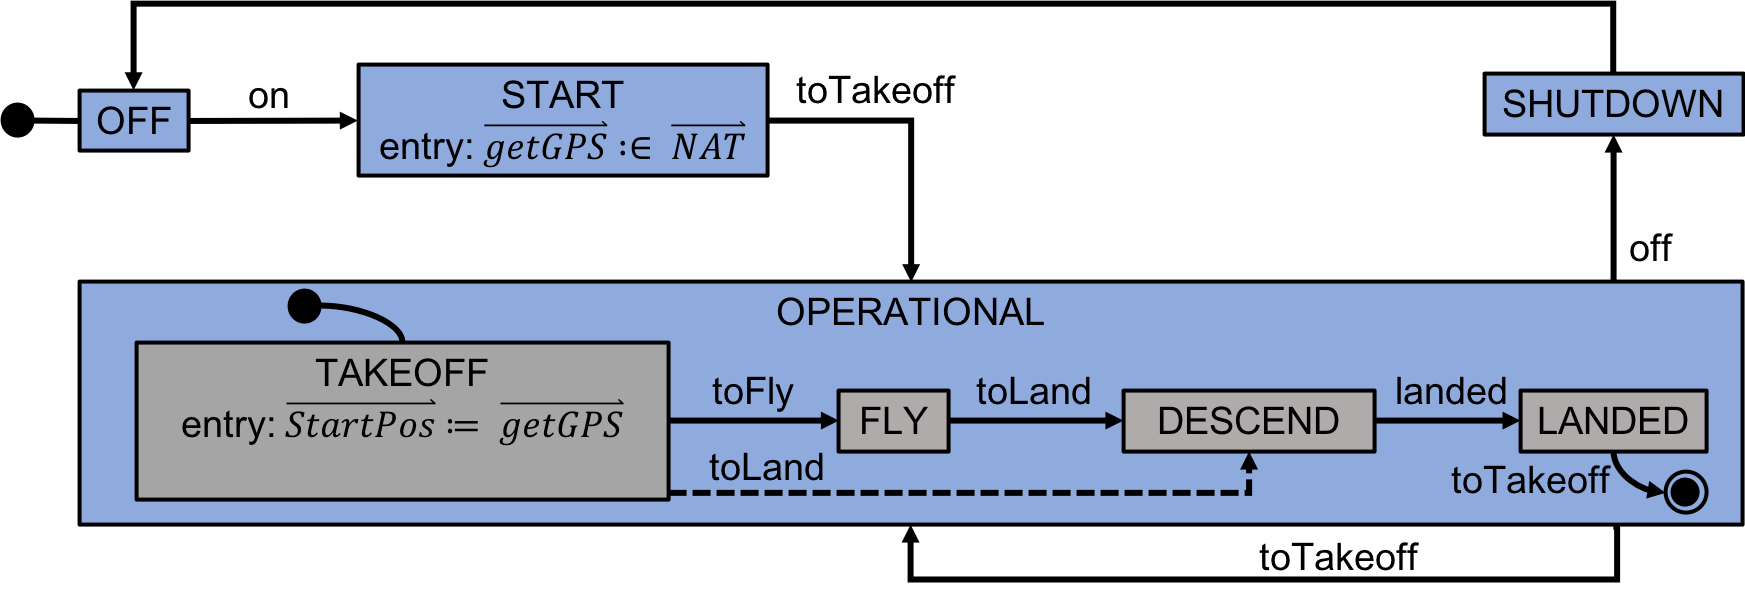
\includegraphics[width=0.90\textwidth, trim=0 40 0 0]{figures/Picture1.png}
	\caption{State-chart of drone application. Abstract level including only generic start/shutdown behavior (shown in blue). The first refinement introducing main operational sub-states, is shown in gray. }
	\label{fig:drone1}
	\vspace{-.4cm}
\end{figure} 


% Figure~\ref{fig:drone2} shows the first refinement of the model, as we refine the parent state |TAKEOFF|
% by introducing child states and new model variables, similar to 
% Rule 2 \emph{basic-to-or state rule} defined by Syriani et al.~\cite{Syriani_2019}
% As part of this refinement we introduced an untriggered transition responsible for 
% raising the |toFly| internal trigger, and therefore removed some of the non-determinisms in the abstraction.

% \begin{figure}[!h]
% 	\centering
% 	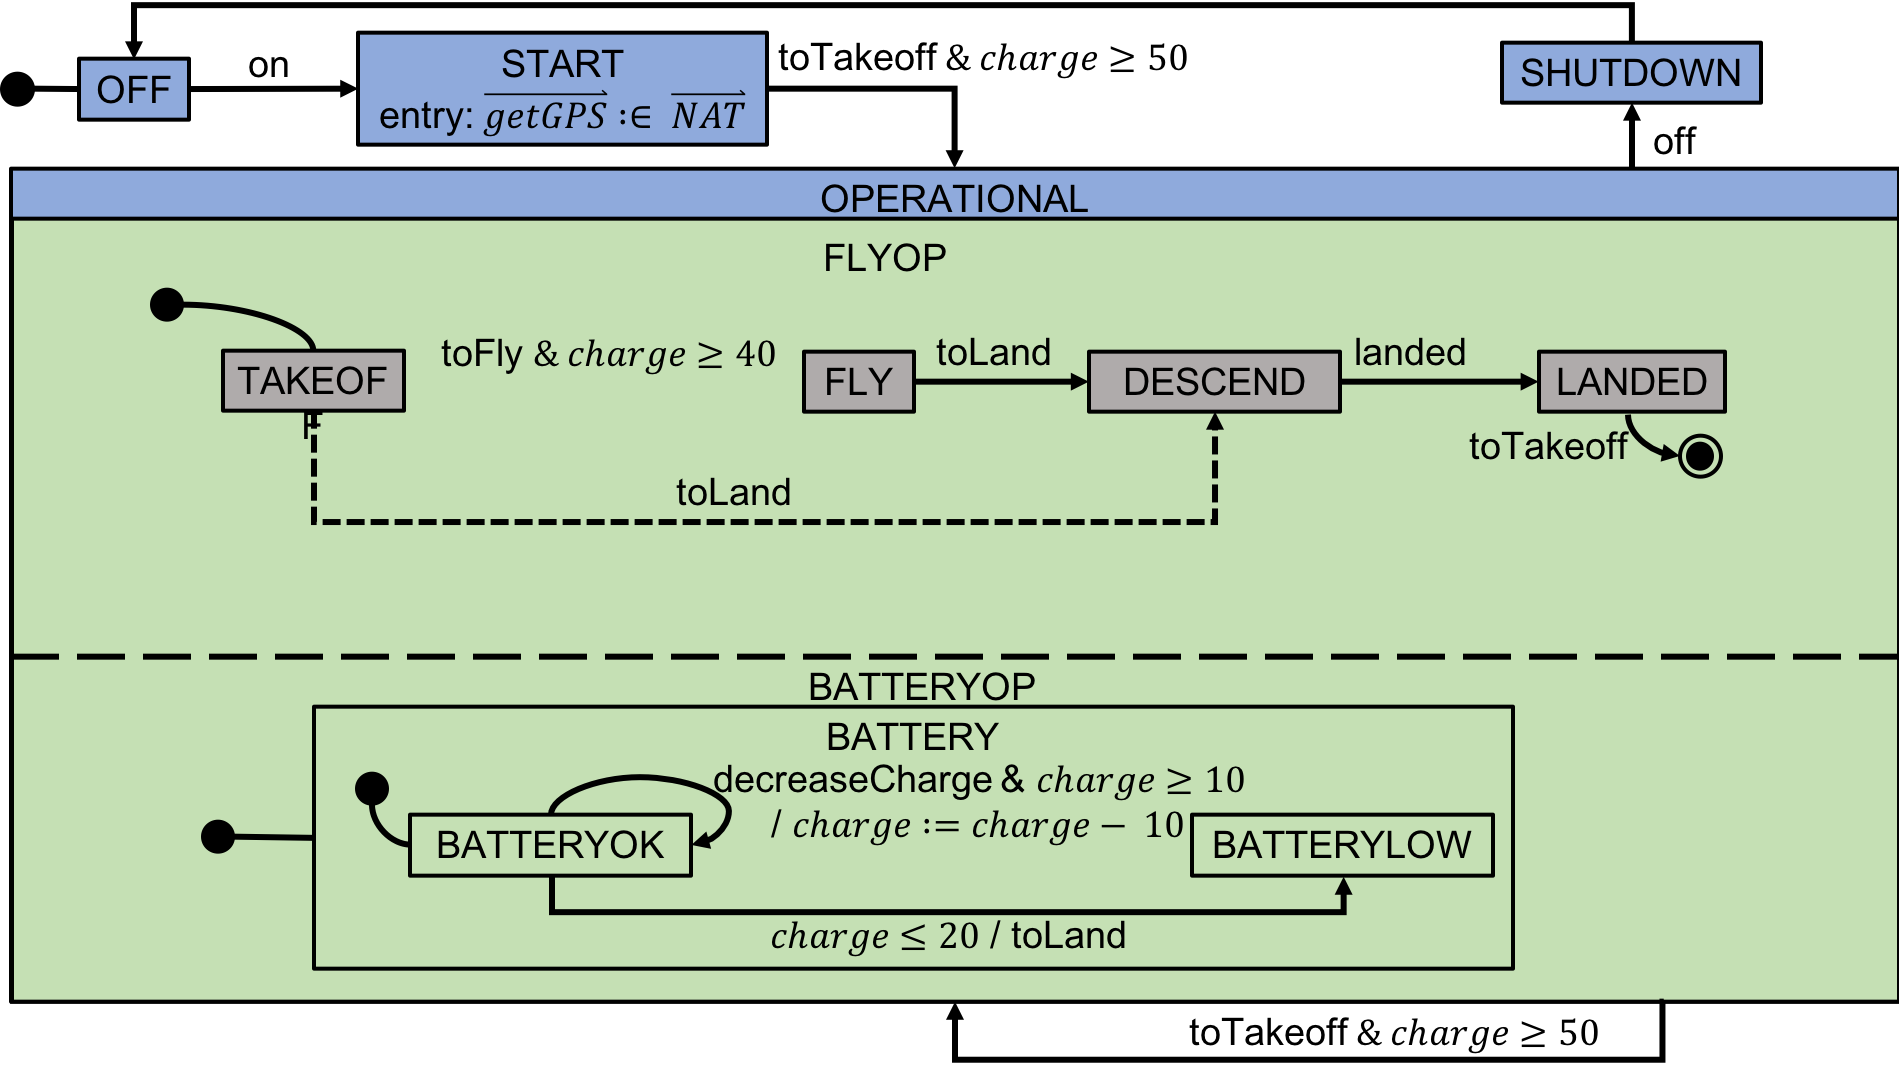
\includegraphics[width=0.95\textwidth]{figures/Picture2.png}
% 	\caption{State-chart of drone application. Refinement level introducing details for take off.}
% 	\label{fig:drone2}
% \end{figure} 
% \begin{figure}[!h]

\begin{figure}[]
	\centering
	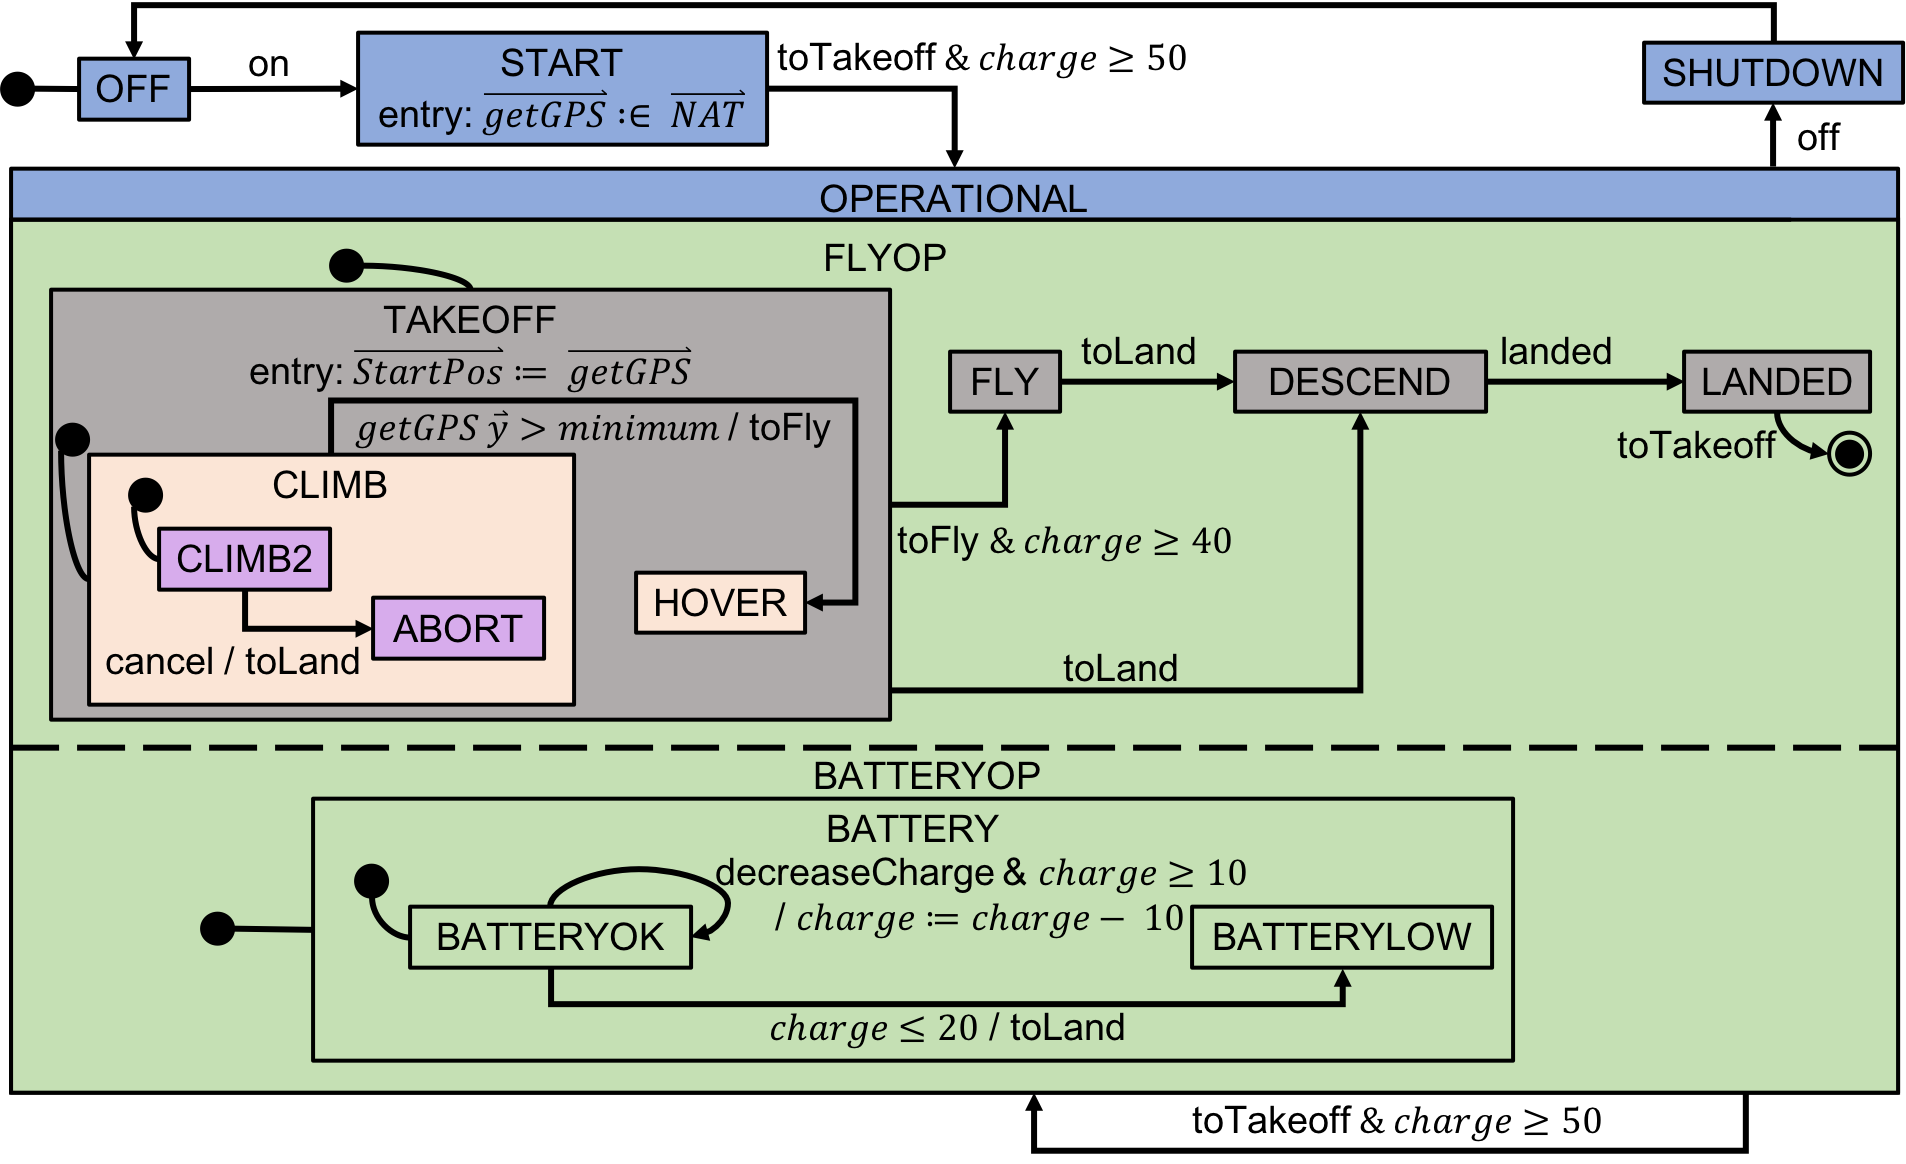
\includegraphics[width=0.90\textwidth, trim=0 30 0 0]{figures/Picture5.png}
	\caption{State-chart of drone application. 
		2nd refinement for battery monitoring functionality (shown in green).
		3rd refinement introducing details for take off (shown in beige).
		4th refinement level to allow cancelling during take-off (shown in lilac).}
	\label{fig:drone4}
\end{figure} 

Figure~\ref{fig:drone4} builds on Figure~\ref{fig:drone1} to show three more refinements to the drone model. 
% Figure~\ref{fig:drone4} shows two subsequent refinements to the drone model.
The second refinement (shown in green in Figure~\ref{fig:drone4}) extends the capabilities within |OPERATIONAL| by using \emph{Rule C} to make it a parallel state that controls flying and battery related functionality. 
This is the same as Rule 4 \emph{and-state rule} defined by Syriani et al.~\cite{Syriani_2019}.
The charge within the drone battery is monitored by the parallel |BATTERYOP| state. 
A new ancillary variable, |charge|, is introduced to keep track of the amount of charge left in the drone.
It is decreased by a self-transition on state |BATTERYOK| in response to an external trigger |decreaseCharge|. 
%As part of this design stage we introduce a requirement to constrain drone flying operation to a battery charge of at least 20\% capacity.
If the battery monitor works correctly we would expect the battery charge to have at least 20\% capacity while in the state |BATTERYOK|.
This can be expressed as an invariant property:
\begin{center}
	|(BATTERYOK = TRUE) => charge > 20|\% .
\end{center}
When the monitored charge drops to 20\% or less, the |BATTERY| state-chart raises the internal trigger |toLand|, which will cause a reaction in the |FLYOP| start-chart to bring it out of |TAKEOFF| or |FLY| and into |DESCEND| (hence removing some of the non-determinism concerning where |toLand| is raised).
While in the |TAKEOFF| state we would expect the battery monitor to be in the |BATTERYOK| state or to have raised a |toLand| trigger.
\begin{center}
	|(TAKEOFF = TRUE) => (BATTERYOK = TRUE ∨ toLand)|~.
\end{center}
%The aforementioned trigger, is raised non-deterministically by some unspecified internal functionality .
%Our state-chart semantics supports transition refinement, which allows us to modify previously defined transitions, by adding guards \emph{Rule A} and/or actions \emph{Rule B} that modify new variables that contribute implementation details to the model. 
To ensure the drone only enters |TAKEOFF| or |FLY| with enough battery power we strengthen the guards of transitions to the |FLY| and |TAKEOFF| states (\emph{Rule A}).
We will discuss how these state invariant properties are verified in Section~\ref{sec:verificationSafety}.

% \begin{figure}[!h]
% 	\centering
% 	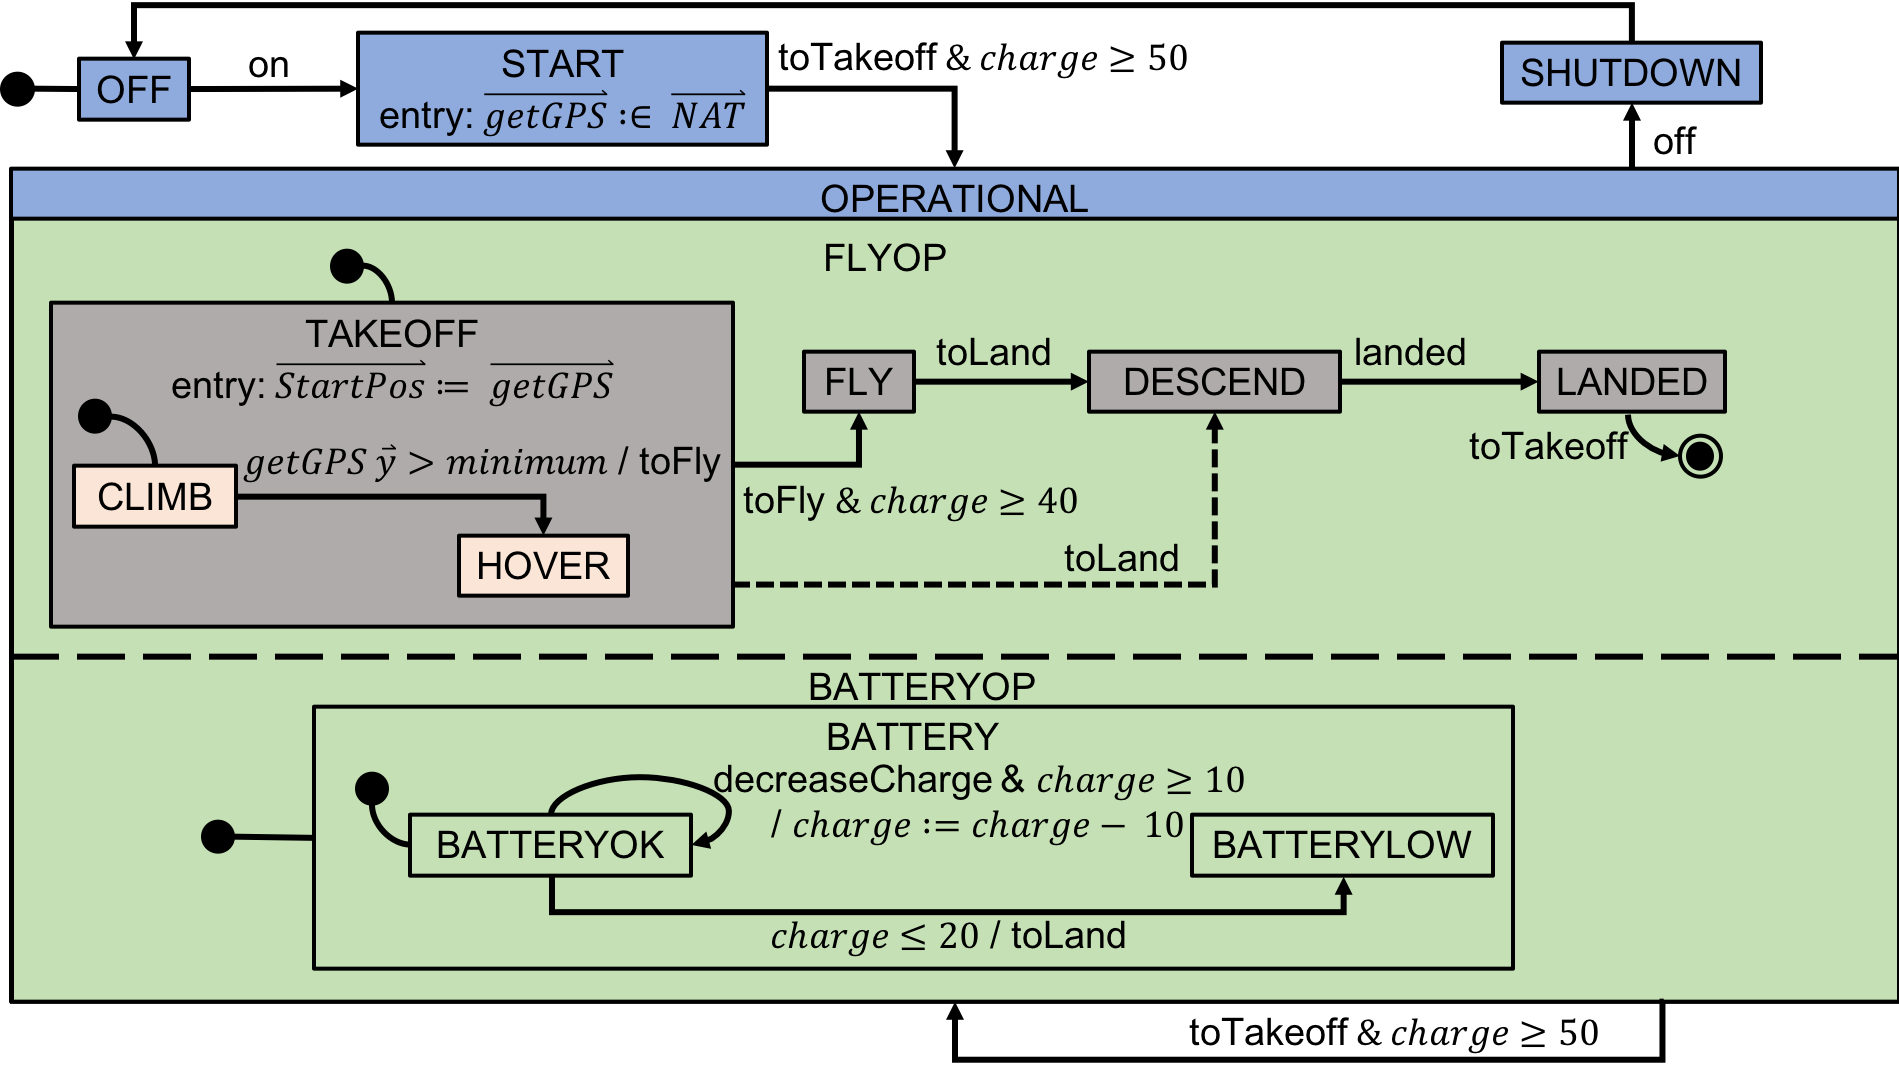
\includegraphics[width=0.95\textwidth]{figures/Picture3.png}
% 	\caption{State-chart of drone application.Refinement level for descending capabilities}
% 	\label{fig:drone3}
% \end{figure} 

The third refinement of the model (shown in beige) refines the state |TAKEOFF| by applying \emph{Rule B and C}. 
Under these rules we introduce child states and new model variables, similar to Rule 2 \emph{basic-to-or state rule} defined by Syriani et al.~\cite{Syriani_2019}
As part of this refinement we introduced an untriggered transition responsible for raising the |toFly| internal trigger, and therefore removed some of the non-determinisms concerning this trigger.

The fourth refinement of the drone model (shown in lilac) uses \emph{Rule C} to introduce additional implementation details to 
allow a take-off to be cancelled in response to an external trigger |cancel|.
%ensure that under special 
%circumstances (e.g.,sensing of adverse environment or unexpected battery dropped) the drone is able 
%to circumvent flying and proceed to an emergency landing. The previously described requirement can be
%expressed as
%\begin{center}
%  |(TAKEOFF = TRUE) => (BATTERYOK = TRUE ∨ toLand)|~.
%\end{center}
%To implement this new capability in the design the internal trigger |cancel| is introduced.
%The internal trigger |cancel| can be raised non-deterministically by some sensing capability, 
%the details of which are not currently implemented. 
If the trigger is raised, the climbing process must be aborted and the drone descending sequence shall start. 
This refinement level is done differently to Syriani et al.~\cite{Syriani_2019}, which follows Rule 7 \emph{state extension rule}. 
The aforementioned rule requires a data remapping of the abstract states |TAKEOFF|, |CLIMB| and |HOVER|, which should be distinct from the states in this  refinement, as the state |ABORT| is introduced.
In contrast, we implement this refinement using a rule similar to Syriani et al.'s  Rule 2 \emph{basic-to-or state rule}, which introduces the concrete states |CLIMB2| and |ABORT| to the abstract state |CLIMB|.

Although the autonomous drone example in this paper is based on the
example described in~\cite{Syriani_2019}, the definition of refinement
used in that work is quite different from our own. This forces some
differences in our refinement rules and consequently the way the
example is developed.  In~\cite{Syriani_2019} ``refinement'' is a
transformation of the model which preserves reachability of a state
with respect to sequences of inputs. However, this also allows the
possibility of introducing new behaviors in the concrete model that
the abstraction does not exhibit. While this notion of refinement
seems useful in certain contexts, unlike refinement in \EventB it does
not guarantee preservation of safety properties. Therefore it should
be considered less suited to development of safety-critical systems.

% Syriani et al. refinement rules
% Rule 1 \emph{action rule}
% Rule 2 \emph{basic-to-or state rule}
% Rule 3 \emph{or-to-and state rule}
% Rule 4 \emph{and-state rule}
% Rule 5 \emph{transition rule}
% Rule 6 \emph{fork rule}
% Rule 7 \emph{state extension rule}
% Rule 8 \emph{path refinement rule}

% Event-B refinement rules
% https://www3.hhu.de/stups/handbook/rodin/current/html/generated_proof_obligations.html
% guard strengthening
% action simulation
% equality of a preserved variable
% guard strengthening (merge)
% well definedness of a witness
% feasibility of witness
% decreasing of variant

%%% Local Variables:
%%% mode: latex
%%% TeX-master: "../main"
%%% End:
